\section{Introduction}
\label{sec:introduction}
\section{Results \& Discussion}
\subsection*{Geometric Representation of Cellular Automata Rules}

Cellular automata (CA) are grid-based computational models where each cell evolves over time according to a rule set \( R \). In Elementary Cellular Automata (ECA), the domain is one-dimensional and the state space is binary, \( S = \{0, 1\} \). Each cell's future state is determined by its current state and those of its immediate neighbors.

Mathematically, for cell \( i \) at time \( t \), the next state \( u_i^{t+1} \) is governed by a rule function \( f: S^3 \to S \):

\[
u_i^{t+1} = f(u_{i-1}^t, u_i^t, u_{i+1}^t)
\]

With a binary state and 3-cell neighborhood, there are \( 2^8 = 256 \) unique ECA rules. These are indexed from 0 to 255, following Wolfram's convention.

For example, Rule 110 is defined as:

\[
f_{\text{110}}: (0,0,0) \to 0, \; (0,0,1) \to 1, \; \ldots, \; (1,1,1) \to 0
\]




\begin{figure}[h]
    \centering
    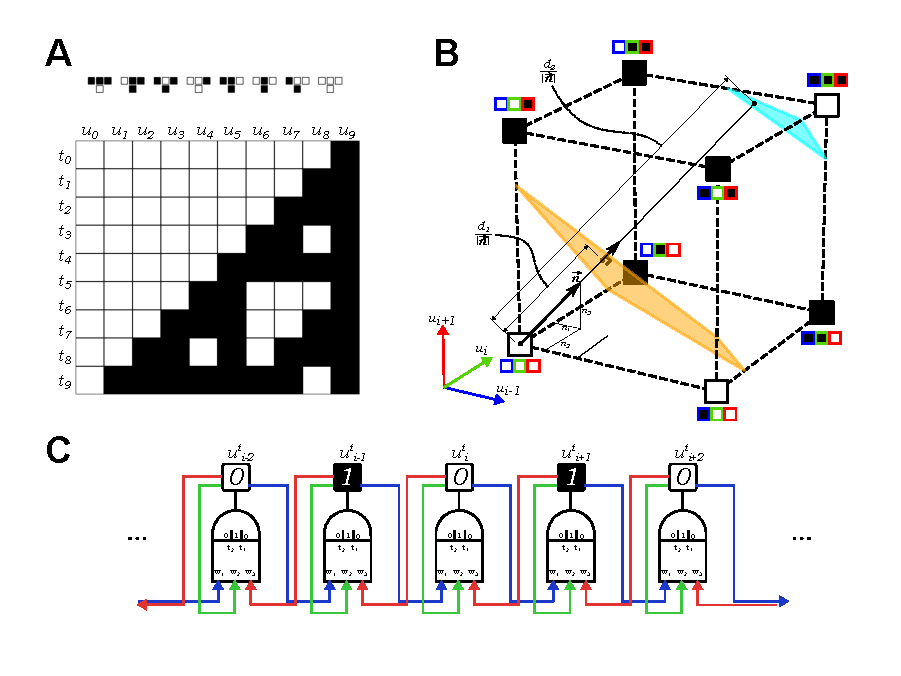
\includegraphics[width=\textwidth]{images/SVGs/Cube.pdf}
    \caption{A. The transition rule and time evolution of the Rule 110 cellular automata. B. Cube representation Rule 110 with separating planes defined by normal vector $\overrightarrow{n}$ and offset constants $d_1$ and $d_2$. }
    \label{fig:cube}
\end{figure}

\subsection*{Concept Mechanism}
\begin{figure}[h]
    \centering
    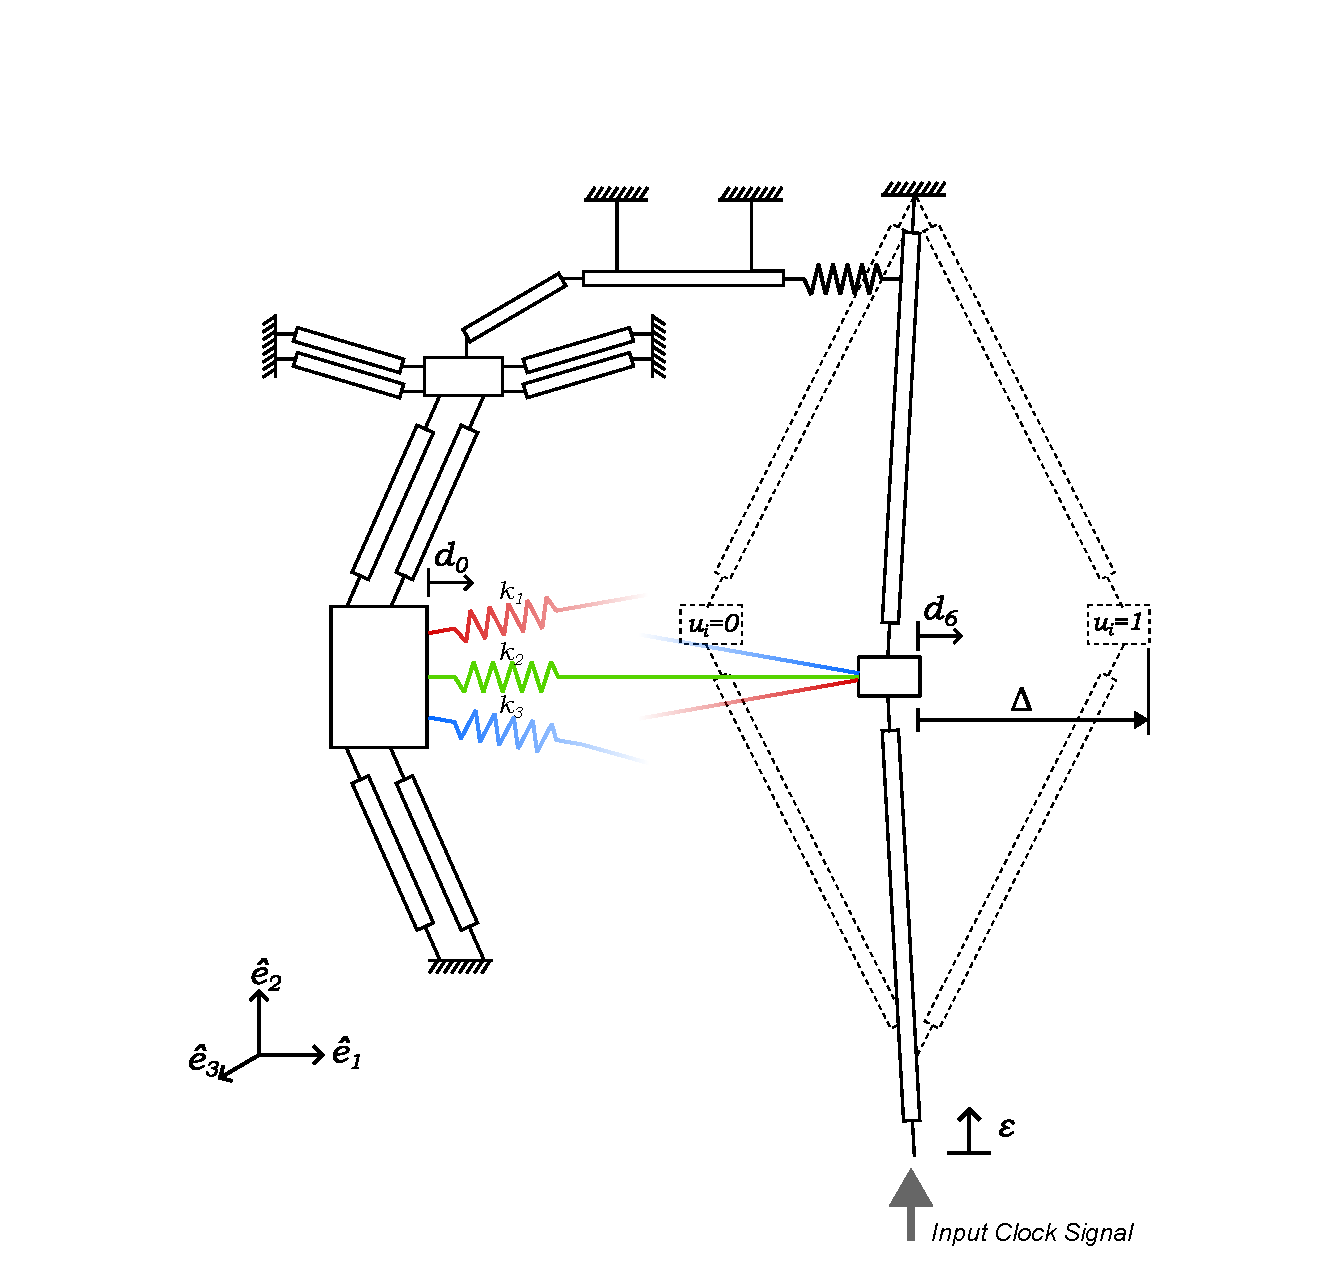
\includegraphics[width=\textwidth]{images/SVGs/PRBM.pdf}
    \caption{This is a figure.}
    \label{fig:Mechanism}
\end{figure}

\begin{figure}[h]
    \centering
    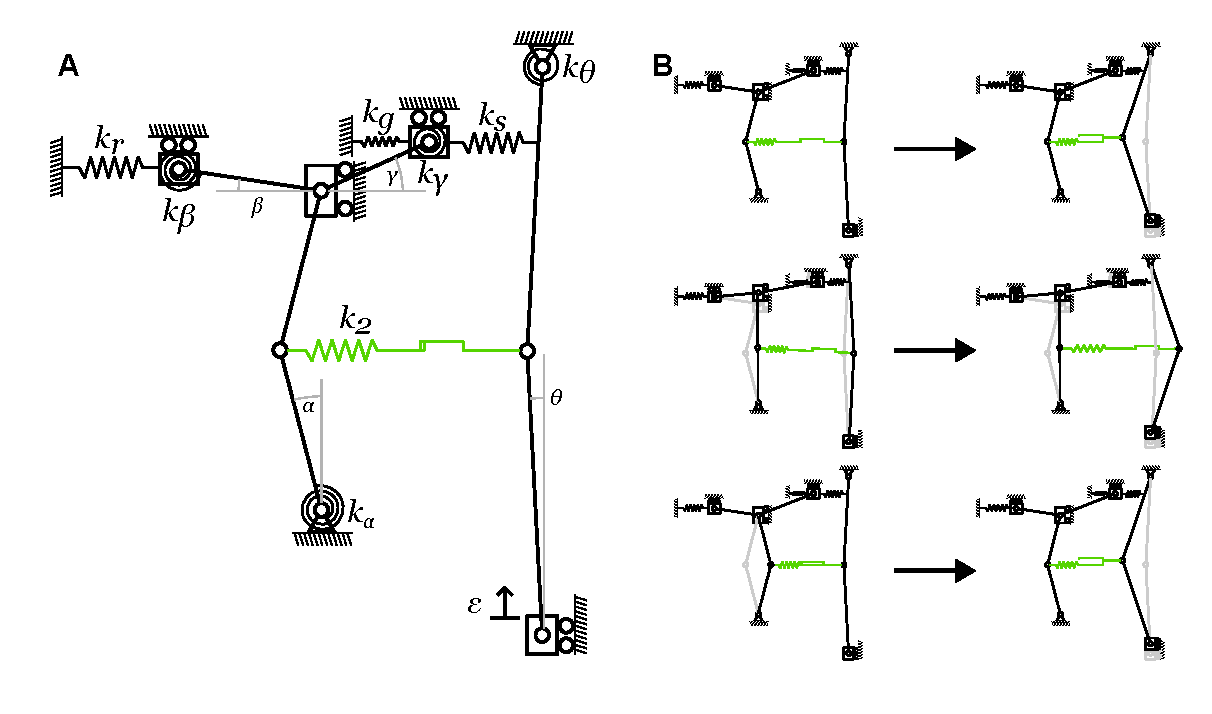
\includegraphics[width=\textwidth]{images/SVGs/Bifurcation_and_PRBM.pdf}
    \caption{This is a figure.}
    \label{fig:Bifurcation}
\end{figure}

\subsection*{Working Principle}
\begin{figure}[h]
    \centering
    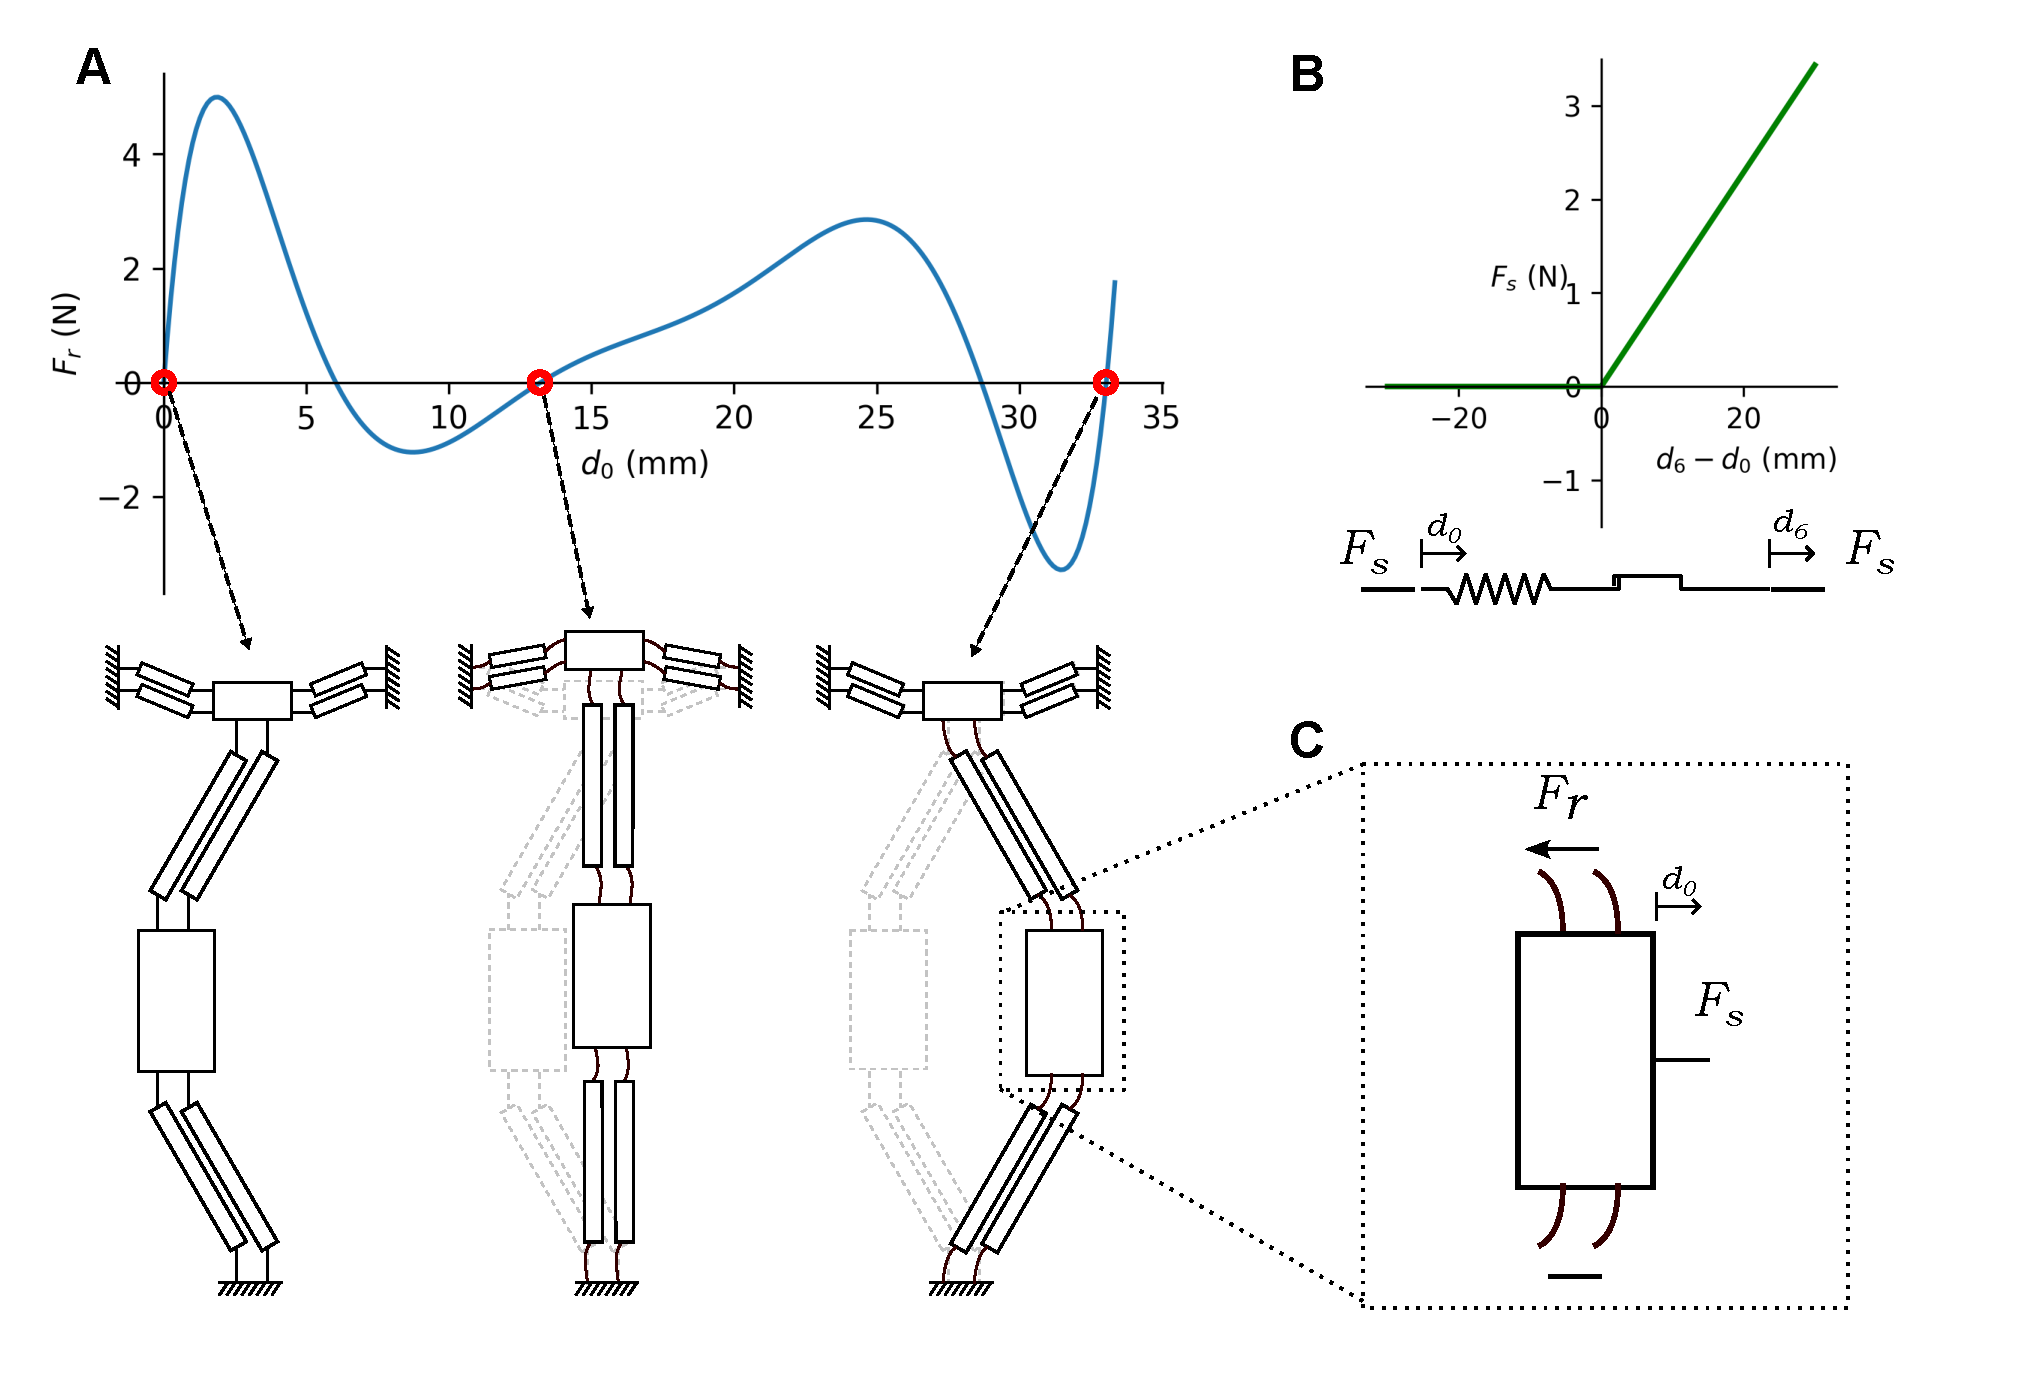
\includegraphics[width=\textwidth]{images/SVGs/Equilibria1.pdf}
    \caption{This is a figure.}
    \label{fig:Equilibria and Tension-only spring}
\end{figure}

\begin{figure}
    \centering
    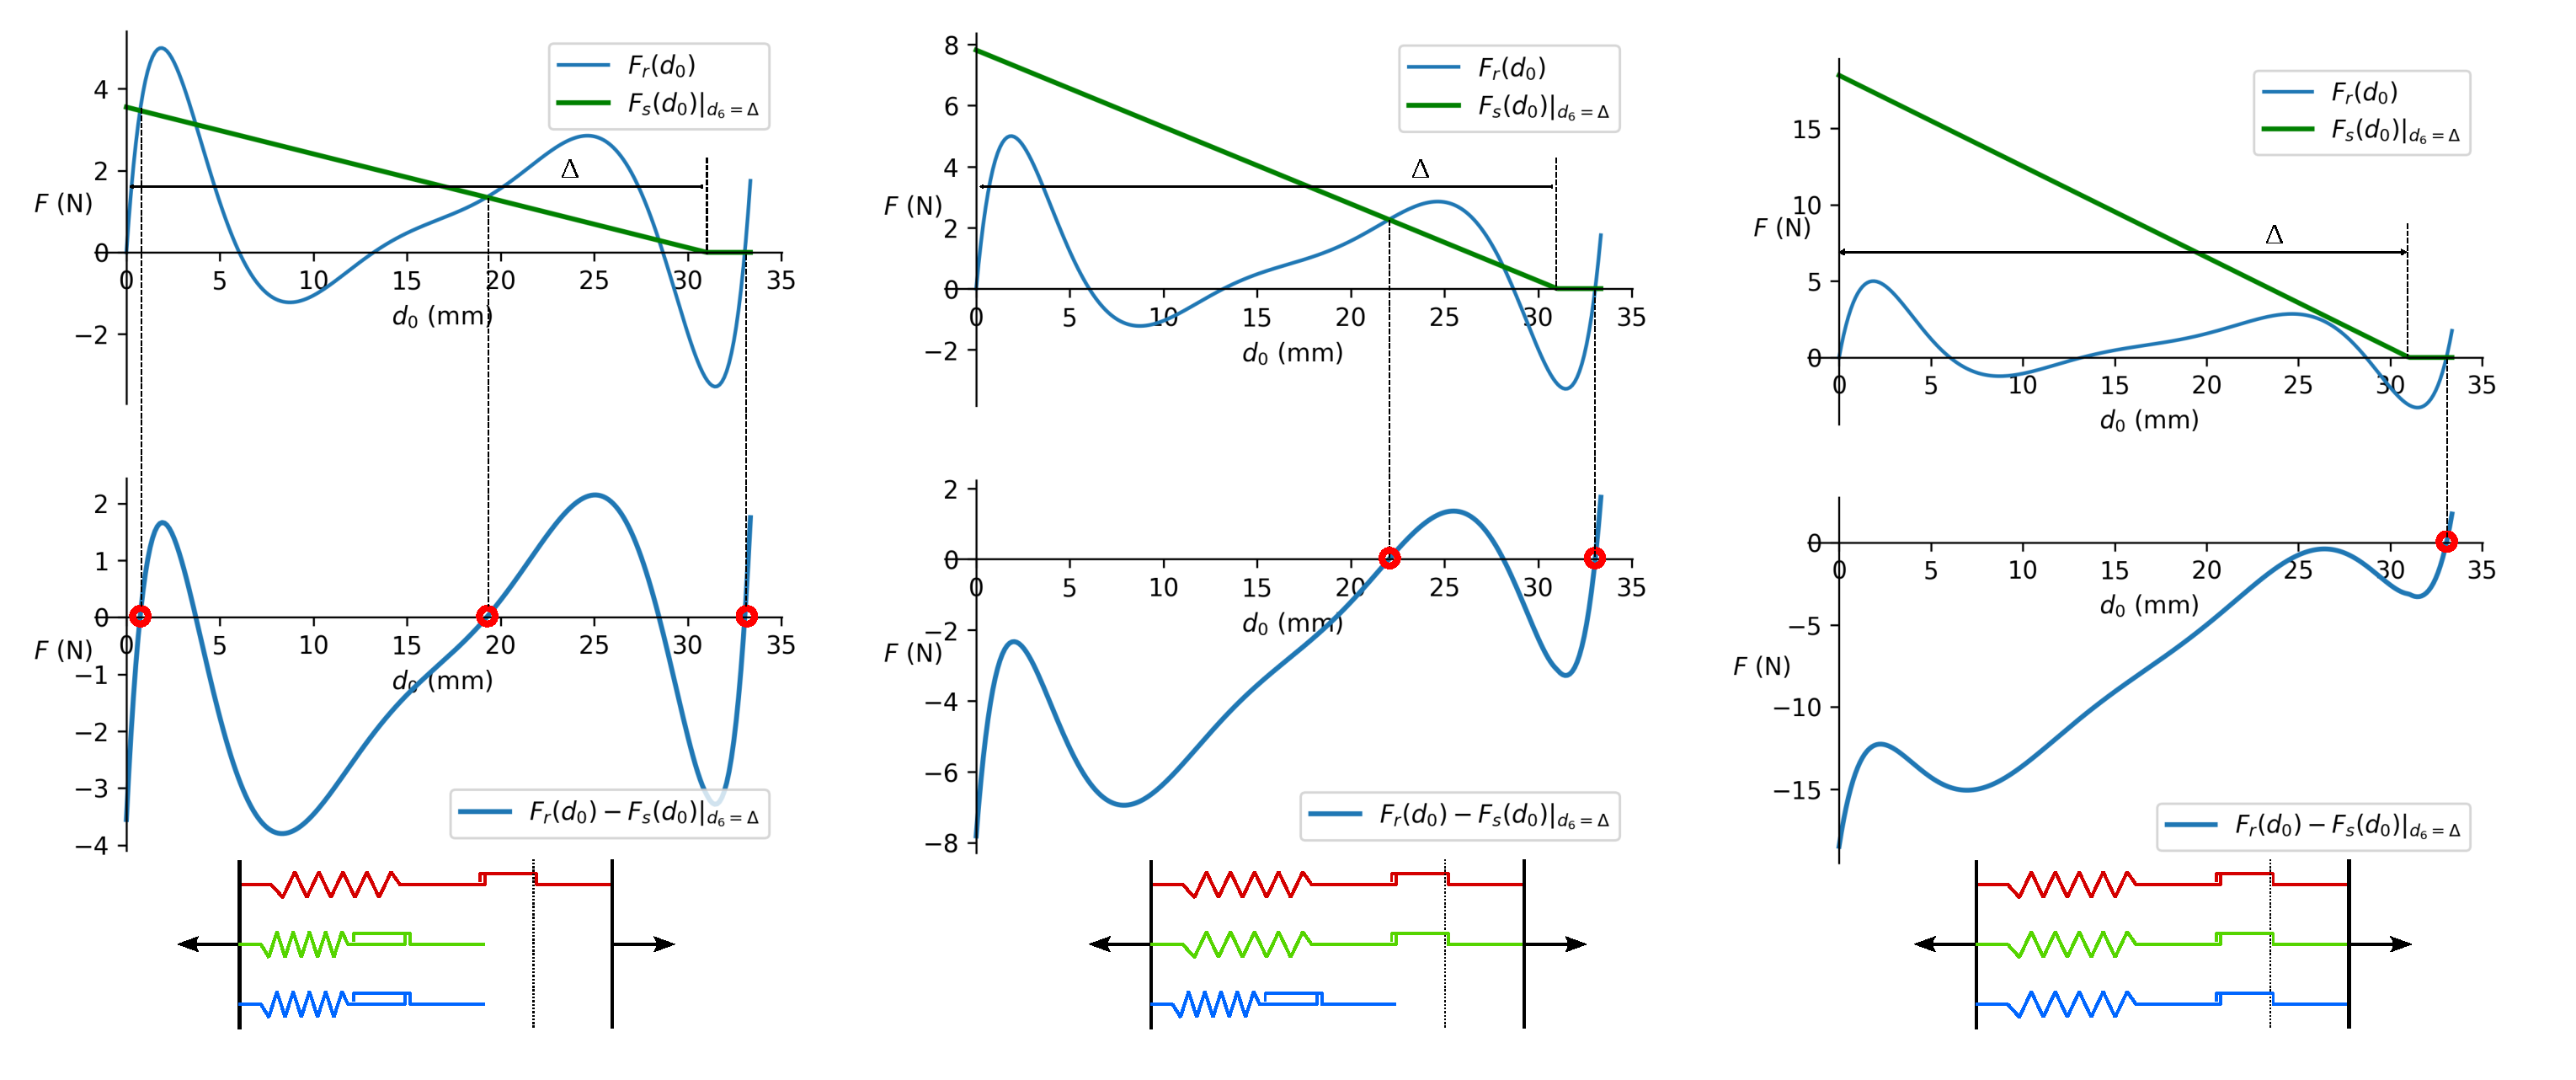
\includegraphics[width=\textwidth]{images/SVGs/Equilibria2.pdf}
    \caption{This is a figure.}
    \label{fig:Equilibria under actuation}
\end{figure}

\begin{figure}
    \centering
    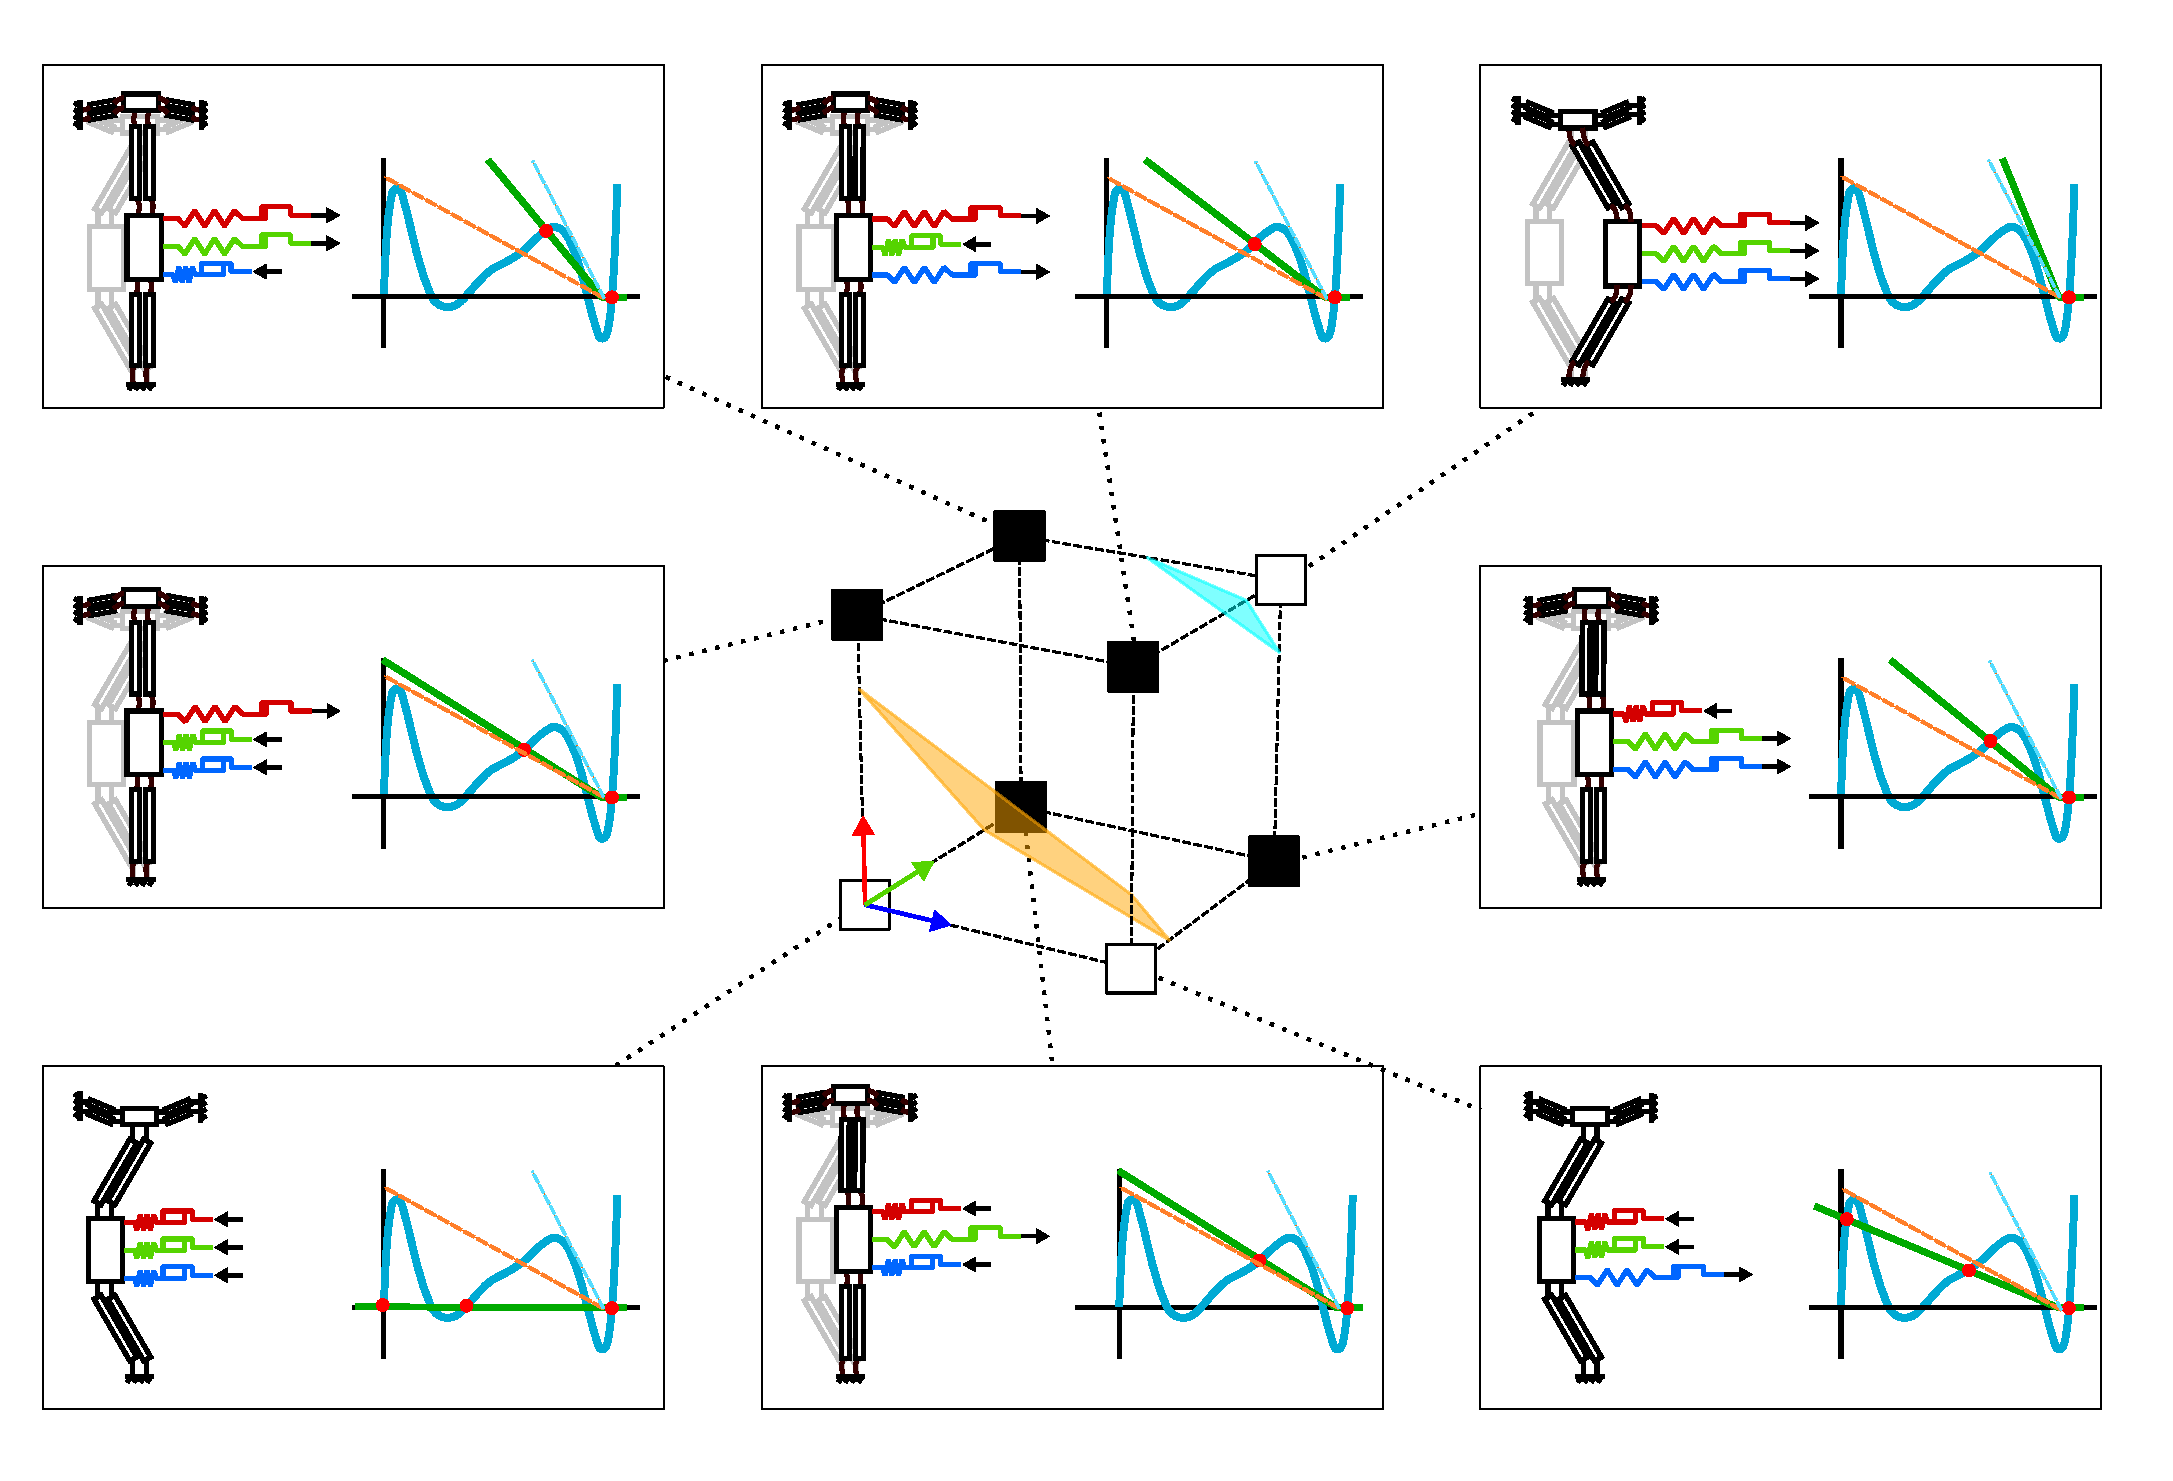
\includegraphics[width=\textwidth]{images/SVGs/Equilibria3.pdf}
    \caption{This is a figure.}
    \label{fig:Equilibria corresponding to Rule 110}
\end{figure}

\subsection*{Simulation}
\section{Conclusion}
\section{References}